\section{Reinforcement Learning}

Reinforcement learning is learning what to do—how to map situations to actions—so as to maximize a numerical reward signal. The learner is not told the correct action to take, but instead must discover which actions yield the most reward by trying them. Actions may affect not only the immediate reward but also the next situation and, through that, all following rewards. The idea that we learn by interacting with our environment is a very intuitive one. Whether we are learning to drive a car or to hold a conversation, we are aware of how our environment responds to our actions, and we want to control what happens through our behavior \cite{sutton_barto_2012}.

A learning problem involves interaction between an active decision-making agent and its environment, in which the agent tries to achieve a goal despite facing uncertainty about its environment. The agent’s actions are allowed to affect the future state of the environment, thereby affecting the options and opportunities available to the agent at later times. Correct choice requires taking into account not only the direct effect of the choice, but also indirect, delayed consequences of actions.

All these features are a good fit to modelling an elevator controller task. Note that we use the word controller instead of agent here, but they are interchangeable. The controller is able to sense the state of its environment, which can be described by the elevator's position and which buttons are pressed, among others. The controller is taking sequential actions that affect the position of the elevator, thereby affecting the state of the environment. The controller's goal is to serve passengers as quickly as possible. Its goals relate to the state of the environment.

\subsection{Exploration and Exploitation}

A fundamental challenge that arises in reinforcement learning is the trade-off between exploration and exploitation. To obtain a high reward, an agent must choose actions that it has tried in the past and found to yield a higher reward than others. It must exploit the knowledge gained from past actions. However, to discover such actions, it has to keep exploring and try actions it has not tried before. An appropriate balance between exploration and exploitation is necessary. Usually this is done as follows. At the start of training, exploratory actions are highly encouraged. As training moves along, we gradually decrease the probability of taking an exploratory action.  

\subsection{Elements of Reinforcement Learning}

Besides the agent and the environment, there are four important subelements in a reinforcement learning system: a policy, a reward signal, a value function, and, optionally, a model of the environment. Their functions will be addressed in this section.

A model of the environment describes the (probabilistic) behavior of the environment. It allows for predictions about the environment’s behavior to be made. For example, given a state and action, the model might predict the next state and next reward.

\subsection{Markov Decision Process}

The concepts of reinforcement learning, continuous interaction between an agent and its environment, are formalized as a Markov decision process (MDP). The agent selects actions using some strategy and the environment reacts by presenting the agent new situations. The environment also emits rewards. The agent seeks to maximize its rewards over time by adapting its strategy. See figure \ref{fig:agent_environment}.

\begin{figure}[H]
    \centering
    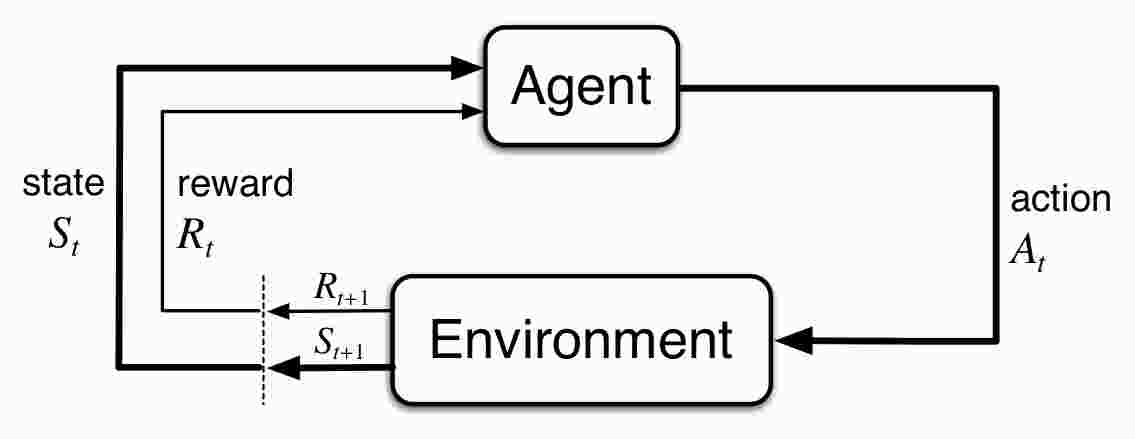
\includegraphics[width=0.8\textwidth]{agent_environment.png}
    \caption{The agent-environment interaction in a Markov decision process \cite{sutton_barto_2012}.}
    \label{fig:agent_environment}
\end{figure}

In a discrete-time MDP, the agent and environment interact at each of a sequence of discrete time steps, $t = 0, 1, 2, 3, \dots$. At each time step $t$, the agent receives some representation of the environment’s state, $S_t \in \S$, and selects an action, $A_t \in \mathcal{A}(s)$ depending on the observed state. One time step later, partly as a result of its action, the agent receives a reward, $R_{t+1} \in \mathcal{R} \subseteq \mathbb{R}$, and finds itself in a new state, $S_{t+1}$. 

In a finite MDP, the sets of states, actions, and rewards ($\mathcal{S}$, $\mathcal{A}$, and $\mathcal{R}$) all have a finite number of elements. In this case, the random variables $R_t$ and $S_t$ have a well defined discrete probability distributions dependent only on the previous state and action. That is, for particular values of these random variables, $s' \in \mathcal{S}$ and $r \in \mathcal{R}$, the probability of those values occurring at time $t$ given values of the previous state and action is given by
\[
    p(s', r | s, a) \coloneqq \Pr(S_t = s' , R_t = r | S_{t-1} = s, A_{t-1} = a)
 \]
for all $s' \in \S$, $r \in \mathcal{R}$, and $a \in \mathcal{A}(s)$. 

The probabilities given by the function $p$ completely determine the dynamics of a finite MDP. From it, anything else we might want to know about the environment, such as the state-transition probabilities $p(s' | s, a)$, can be computed.

\subsection{Returns}

A reward signal defines the goal in a reinforcement learning problem. The reward signal thus defines what the good and bad events for the agent are. The agent’s objective is to maximize the total reward it receives over the long run. If an action selected by the policy is followed by low reward, the policy may be changed to select some other action in that same situation in the future.

Let $R_{t+1}, R_{t+2}, R_{t+3}, \dots$ denote the sequence of rewards received after time step $t$. Generally, we want to maximize the expected return $G_t$, which is some specific function of the reward sequence. For our specific task, we define this to be the sum of discounted future rewards
\begin{equation}
    G_t \coloneqq R_{t+1} + \gamma R_{t+2} + \gamma^2 R_{t+3} + \cdots = \sum_{k=0}^{\infty} \gamma^{k}R_{t+k+1} \label{eq:returns}
\end{equation}

where $\gamma \in [0,1]$ is a parameter called the \textit{discount rate}.

The discount rate determines the present value of future rewards: a reward received $k$ time steps in the future is worth only $\gamma^{k-1}$ times what it would be worth if it were received immediately. If $\gamma < 1$, the infinite sum in (\ref{eq:returns}) has a finite value as long as the reward sequence $\{R_k\}$ is bounded. As $\gamma$ approaches 1, the objective takes future rewards into account more strongly.

Returns at successive time steps are related recursively:
\begin{align*}
    G_t &\coloneqq R_{t+1} + \gamma R_{t+2} + \gamma^2 R_{t+3} + \gamma^3 R_{t+4} + \cdots \nonumber\\
    &= R_{t+1} + \gamma (R_{t+2} + \gamma R_{t+3} + \gamma^2 R_{t+4} + \cdots) \nonumber\\
    &= R_{t+1} + \gamma G_{t+1}.
\end{align*}

\subsection{Policies}

A policy defines the learning agent’s way of behaving, i.e. which actions it selects, at a given time. Roughly speaking, a policy is a mapping from states of the environment to actions to be taken when in those states. The policy alone is sufficient to determine the agent's behavior.

Formally, a policy $\pi$ is a mapping from states to a probability distribution over the possible actions that can be selected in those states. If the agent is following policy $\pi$ at time $t$, then $\pi(a \cbar s)$ is the probability that $A_t = a$ if $S_t = s$. Reinforcement learning methods specify how the agent’s policy is changed as a result of its experience.

\subsection{Value Functions}

The value of a state $s$, $v(s)$, is the return that the agent is expected to acquire in the future, starting from that state. Whereas rewards determine the immediate benefit of an environmental state, values indicate the long-term desirability of states after taking into account the states that are likely to follow, and the rewards available in those states. For example, a state might always yield a low immediate reward but still have a high value because it is often followed by other states that yield high rewards.

The value of a state $s$ under a policy $\pi$, denoted $v_\pi(s)$, is the expected return when starting in $s$ and following $\pi$ thereafter. For MDPs, we can define $v_\pi$ formally by
\begin{equation}
    v_\pi(s) \coloneqq \E_\pi[G_t \cbar S_t = s] = \E_\pi\left[\sum_{k=0}^{\infty} \gamma^k R_{t+k+1} \bigbar S_t = s\right], \text{ for all } s \in S
\end{equation}
    
where $\E_\pi[\cdot]$ denotes the expected value of a random variable given that the agent follows policy $\pi$, and $t$ is any time step. We call the function $v_\pi$ the state-value function for policy $\pi$.
Similarly, we define the value of taking action $a$ in state $s$ under a policy $\pi$, denoted $q_\pi(s, a)$, as the expected return starting from $s$, taking the action $a$, and thereafter following policy $\pi$:

\begin{equation}
    q_\pi(s, a) \coloneqq \E_\pi[G_t \cbar S_t = s, A_t = a] = \E_\pi\left[\sum_{k=0}^{\infty} \gamma^k R_{t+k+1} \bigbar S_t = s, A_t = a\right].
\end{equation}

We call $q_\pi$ the action-value function for policy $\pi$. If all the dynamics of an environment were completely specified, exact value functions could be computed. If that were not the case, the value functions $v_\pi$ and $q_\pi$ would have to be estimated from (simulated) experience. The first is called a model-based approach, while the latter is called model-free. Since the dynamics of an elevator system are quite complex, we adopt the model-free approach.

Of course, if there are a lot of states, it may not be practical to keep around values for each state individually. The agent would have to parameterize the value functions $v_\pi$ and $q_\pi$ (with fewer parameters than states) and adjust the parameters to better match the observed returns. Linear models and artificial neural networks are often used in this case. Similar states would then get similar values. This can also produce accurate estimates, depending on the approximation function. We try to keep the state space small enough to allow for use of tabular methods, since approximate solutions are a bit more complex to analyze.

For any policy $\pi$ and any state $s$, the following condition holds between the value of $s$ and the value of its possible successor states:

\begin{align}
    v_\pi(s) &= \sum_a \pi(a\cbar s) \sum_{s', r} p(s', r \cbar s, a)\Bigr[r + \gamma v_{\pi}(s')\Bigr], \text{ for all } s\in \S 
\end{align}

which are called the Bellman equations for $v_\pi$.

\subsection{Optimality}

Solving a reinforcement learning task means, roughly, finding a policy that achieves a lot of reward over the long run.
A policy $\pi$ is defined to be better than or equal to a policy $\pi'$ if its expected return is greater than or equal to that of $\pi'$ for all states. In other words, $\pi \geq \pi'$ if and only if $v_\pi(s) \geq v_\pi'(s)$ for all $s \in \S$. There is always at least one policy that is better than or equal to all other policies. This is an optimal policy. Although there may be more than one, we denote all the optimal policies by $\pi_*$ . They share the same state-value function, called the optimal state-value function, denoted $v_*$, and defined as
\begin{equation}
    v_*(s) \coloneqq \max\limits_{\pi}v_\pi(s),
\end{equation}
for all $s \in \S$.
Optimal policies also share the same optimal action-value function, denoted $q_* $, and defined as
\begin{equation}
    q_*(s, a) \coloneqq \max\limits_{\pi} q_\pi(s, a),
\end{equation}
for all $s \in S$ and $a \in A(s)$. For the state–action pair $(s, a)$, this function gives the expected return for taking action $a$ in state $s$ and thereafter following an optimal policy.

The optimal value functions $v_*(s)$ and $q_*(s,a)$ can be found by solving the \textit{Bellman optimality equations}. These are given by
\begin{equation}
    v_*(s) = \max\limits_a q_{\pi_*}(s,a) = \max\limits_a \sum_{s', r} p(s', r \cbar s, a) \Bigr[r + \gamma v_*(s')\Bigr]
\end{equation}
for $v_*(s)$, and
\begin{equation}
    q_*(s, a) = \sum_{s', r} p(s', r \cbar s, a) \Bigr[r + \gamma \max\limits_a q_*(s', a)\Bigr]
\end{equation}
for $q_*(s, a)$, for all $s \in \S$ and for all $a \in \mathcal{A}(s)$.

For finite MDPs, a solution to the Bellman optimality equations always exists.

Having $q_*$ makes choosing optimal actions easy. For any state $s$, it can simply find any action that maximizes $q_*(s, a)$. It provides the optimal expected long-term return for each state-action pair. The optimal action-value function allows optimal actions to be selected without having to know anything about the environment’s dynamics.

Many reinforcement learning methods can be seen as approximately solving the Bellman optimality equations, using actual experienced transitions instead of knowledge of the expected transitions. The on-line nature of reinforcement learning makes it possible to approximate optimal policies in ways that puts more effort into learning to make good decisions for frequently encountered states, at the expense of less effort for infrequently encountered states.
